\chapter{Difficultés rencontrées}

Une des difficultés principales de ce projet tenait de l’apprentissage de l’API Android, et de son fonctionnement. L’API Android étant vaste, il n’était pas toujours facile de savoir si nous avions trouvé la solution optimale à un problème donné.\\
Nous avons décidé d'utiliser un \emph{ViewPager} afin de rendre le défilement d’un événement à un autre plus ergonomique. Or pour cela il a fallu implémenter une nouvelle activité. Ceci a légèrement compliqué l'enregistrement des événements comme lus depuis cette activité. Nous avons cherché la meilleure méthode de transmettre des données d’une activité à une autre, et sommes arrivés à la sérialisation d’objets à l'aide des objets de type \emph{Intent}. Cette méthode n'est pas forcément la solution idéale, mais semble être le moyen le plus apte à réaliser le travail nécessaire. \\

Lors de l’implémentation de l’extraction des dates, nous avons rencontré des problèmes concernant l’inclusion des librairies CUP et JFlex. Les méthodes n’étaient pas reconnues au sein du projet, rendant leur utilisation impossible.
Nous avons donc opté pour l'utilisation d'expressions régulières qui reconnaissent des dates. \\

En ce qui concerne les événements, nous avons dû faire comme prévu, deux récupérations d’information différentes, le parsing des flux RSS et le parsing des pages HTML.
Le parsing des flux et des pages a donné lieu à de nouvelles difficultés, notamment concernant les dates. Puisque beaucoup d'événements avaient la mauvaise date, voire même aucune date, nous avons dû essayer de déterminer la date correcte à partir du texte de l'événement. \\

Concernant les pages HTML, nous avons dû comprendre comment étaient organisées celles-ci, quels étaient les éléments à entrer dans la requête afin de récupérer les événements sur une certaine durée. Nous avons utilisé \emph{Jsoup} pour extraire les éléments. Ainsi, étant donné que les pages HTML du LaBRI sont agencées d'une certaine forme, il a fallu adapter le code pour parser ces pages.
Bien que la tâche ne nous fut pas incombée, nous voulions vérifier que les événements étaient complets, afin de ne pas encombrer l'application d'informations incompletes, voire inutilisables. En effet, certains d’eux ne possèdent pas de titre ou de descriptif, ou encore contiennent des informations inutilisables, voire insensées (voir exemple ci-dessous).

\begin{adjustbox}{minipage=1.0\textwidth, margin=0pt \smallskipamount, center}
\begin{lstlisting}[style=HTML, label=htmlCode, caption=Exemple d'événement HTML sans contenu (descriptif vide)]
<table width=100% cellspacing=0 style="border: solid 1px 
   #D3CFC4;">
   <tr>
      <td bgcolor="#c0c0">
         2013-03-21 <!--date-->
      </td>
      <td
         colspan=4 class="surligne">
         <b>
            RENCONTRE P UNG  <!-- titre -->
         </b>
      </td>
   </tr>
   <tr>
      <td width=100 valign=top>
         11:00-12:00        <!-- horaire -->
         <br>SALLE 1278     <!-- lieu -->
      </td>
      <td colspan=4 width=640>
         Intervenant: <br><br>
         <div align=justify>
         <!-- description -->
         </div>
      </td>
   </tr>
   <tr>
      <td></td>
      <td bgcolor=#cccccc width=75 align=center>
      <a href="javascript:openInfosActu('9121', '7371', 'groupe_details', '23', '0');">
         Plus d'infos</a>
      </td>
      <td width=435>&nbsp;<img src="../images/document.gif" title="Documentslies"></td>
</table>
\end{lstlisting}
\end{adjustbox}

\wl Nous avons eu des difficultés avec l’utilisation de \emph{ContentProvider} pour la gestion des événements du calendrier. En effet, selon les modèles de smartphone, l’utilisation de l’API est différente à cause notamment de la surcouche logicielle ajoutée par les constructeurs. Nous avons finalement décidé d’effectuer l’import de l’emploi du temps dans le calendrier par défaut. D’autres difficultés ont également été rencontrées pour insérer tous les événements en une fois (insertion par lots, ou \emph{batch insert}). Mais après plusieurs expérimentations, de multiples recherches et la lecture de nombreux posts sur l’excellent forum StackOverflow, nous sommes parvenu à implémenter cette fonctionnalité. \\

Nous avons également eu quelques soucis pour réceptionner les réponses des requêtes que nous soumettions auprès du serveur LDAP de Bordeaux 1. Le serveur refusait de donner suite aux requêtes renvoyant plus de dix résultats et nous affichait le message d'erreur \textit{size limit exceeded (maximum size is 10)}. C'est donc une restriction imposée par le serveur et il fallait faire avec. Cependant, il fallait tout de même trouver un système pour limiter la taille de nos requêtes à dix éléments pour éviter de lever une \textit{LDAPException} qui nous empêchait d'accéder aux dix premiers contacts retournés. Une recherche plus approfondie au sein de la documentation de la SDK \textit{UnboundID} nous a permis de trouver la solution au problème. \\ 

\begin{figure}[h!]
  \label{fig:simple_paged_results}
  \center
  \setlength\fboxsep{5pt}
  \setlength\fboxrule{0.5pt}
  \fbox{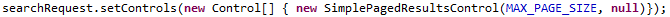
\includegraphics[width=1.0\textwidth]{resources/simplePagedResults.png}}
\end{figure}


L'utilisation du système \emph{Simple paged result control} propre au protocole LDAP nous a permis de demander au serveur de nous renvoyer une seule page de taille \textit{MAX\_PAGE\_SIZE=10} contenant les dix premiers résultats de la requête. Si la recherche effectuée contient donc plus de dix résultats, il seront ignorés à cause des restrictions techniques propres au serveur LDAP en question.